\documentclass[11pt]{a0poster}

\usepackage{url}
\usepackage{graphicx}
\usepackage[usenames,dvipsnames]{color}
\usepackage[margin=0in]{geometry}
\usepackage{xcolor}
\usepackage{graphicx}
\usepackage{amsmath}

\widowpenalty=500
\clubpenalty=500
\fboxsep=0pt

\renewcommand*{\familydefault}{\sfdefault}

\date{}

\begin{document}

\begin{minipage}{0.887\linewidth}
\vspace{100pt}
\hspace{100pt}
\color{Blue}
{\fontsize{3cm}{1em} \textbf{Distributed OLC Genome Assembly With Ananas}}

\hspace{100pt}
\huge Frank Austin Nothaft

\hspace{100pt}
\huge fnothaft@berkeley.edu
\vspace{100pt}
\end{minipage}
\begin{minipage}{0.113\linewidth}
\includegraphics[scale=0.6]{ucseal_540_139.pdf}
\end{minipage}

{\color{Blue}\noindent\makebox[\linewidth]{\rule{\paperwidth}{30pt}}}

\noindent\colorbox{Yellow}{
\begin{minipage}[t][2045pt][t]{\linewidth}

\noindent\begin{minipage}{0.025\linewidth}
\hfill
\pagebreak
\end{minipage}
\begin{minipage}{0.3\linewidth}
\vspace{75pt}
\colorbox{Blue}{
\begin{minipage}{\linewidth}
\vspace{25pt}
\begin{center}
\Huge \bf \color{White} Background
\end{center}
\vspace{10pt}
\end{minipage}
}
\colorbox{White}{
\begin{minipage}[t][600pt][t]{\linewidth}
\color{Blue}
\vspace{20pt}
\LARGE For long reads, genome assembly can be framed using the \textbf{OLC} paradigm:
\begin{enumerate}
\item Find \textbf{overlaps} between all reads
\item \textbf{Layout} these reads in a graph
\item Derive a \textbf{consensus} sequence through the graph
\end{enumerate}
\vspace{20pt}
\textbf{Goals:}
\begin{enumerate}
\item Reduce the cost of overlapping, na\"{i}vely $\mathcal{O}(n^2)$
\item Use commodity map-reduce to distribute graph processing
\item Enable parallel assembly for long read datasets
\end{enumerate}
\hfill
\pagebreak
\end{minipage}
}

\vspace{75pt}
\colorbox{Blue}{
\begin{minipage}{\linewidth}
\vspace{25pt}
\begin{center}
\Huge \bf \color{White} Performance
\end{center}
\vspace{10pt}
\end{minipage}
}
\colorbox{White}{
\begin{minipage}[t][1020pt][t]{\linewidth}
\color{Blue}
\vspace{20pt}
\LARGE
\textbf{Pipeline Performance:}
\begin{itemize}
\item Evaluated on 1.5GB E. coli dataset
\item Evaluated using 2--4 EC2 \texttt{r3.2xlarge} instances
\item Achieve linear speedup
\end{itemize}
\begin{center}
\includegraphics[width=0.45\linewidth]{graphs/speedup.pdf}
\includegraphics[width=0.45\linewidth]{graphs/overlap.pdf}
\end{center}
\textbf{Overlapper Performance:}
\begin{itemize}
\item Overlapper is $\sim$10\% of runtime
\item Runtime degrades with number of buckets used
\item 2$\times$ increase in number of buckets leads to a $2\times$ increase in data size and shuffle volume
\item Na\"{i}ve cartesian product overlapper does not complete
\end{itemize}
\pagebreak
\end{minipage}
}
\pagebreak
\end{minipage}
\begin{minipage}{0.03\linewidth}
\hfill
\pagebreak
\end{minipage}
\begin{minipage}{0.6\linewidth}

\vspace{70pt}
\colorbox{Blue}{
\begin{minipage}[t]{\linewidth}
\vspace{30pt}
\begin{center}
\Huge \bf \color{White} MinHash-Based Overlapping
\end{center}
\vspace{17pt}
\end{minipage}
}
\colorbox{White}{
\begin{minipage}[t][470pt][t]{\linewidth}
\begin{minipage}{0.3\linewidth}
\LARGE
\color{Blue}
\begin{itemize}
\item Overlapping is an all-to-all comparison of reads to see if they contain overlapping sequence
\item However, with proper indexing, we can eliminate many of the read vs. read comparisons
\item We can effectively achieve this by applying LSH to signatures
\end{itemize}
\end{minipage}
\begin{minipage}{0.03\linewidth}
\hfill
\pagebreak
\end{minipage}
\begin{minipage}{0.64\linewidth}
\begin{center}
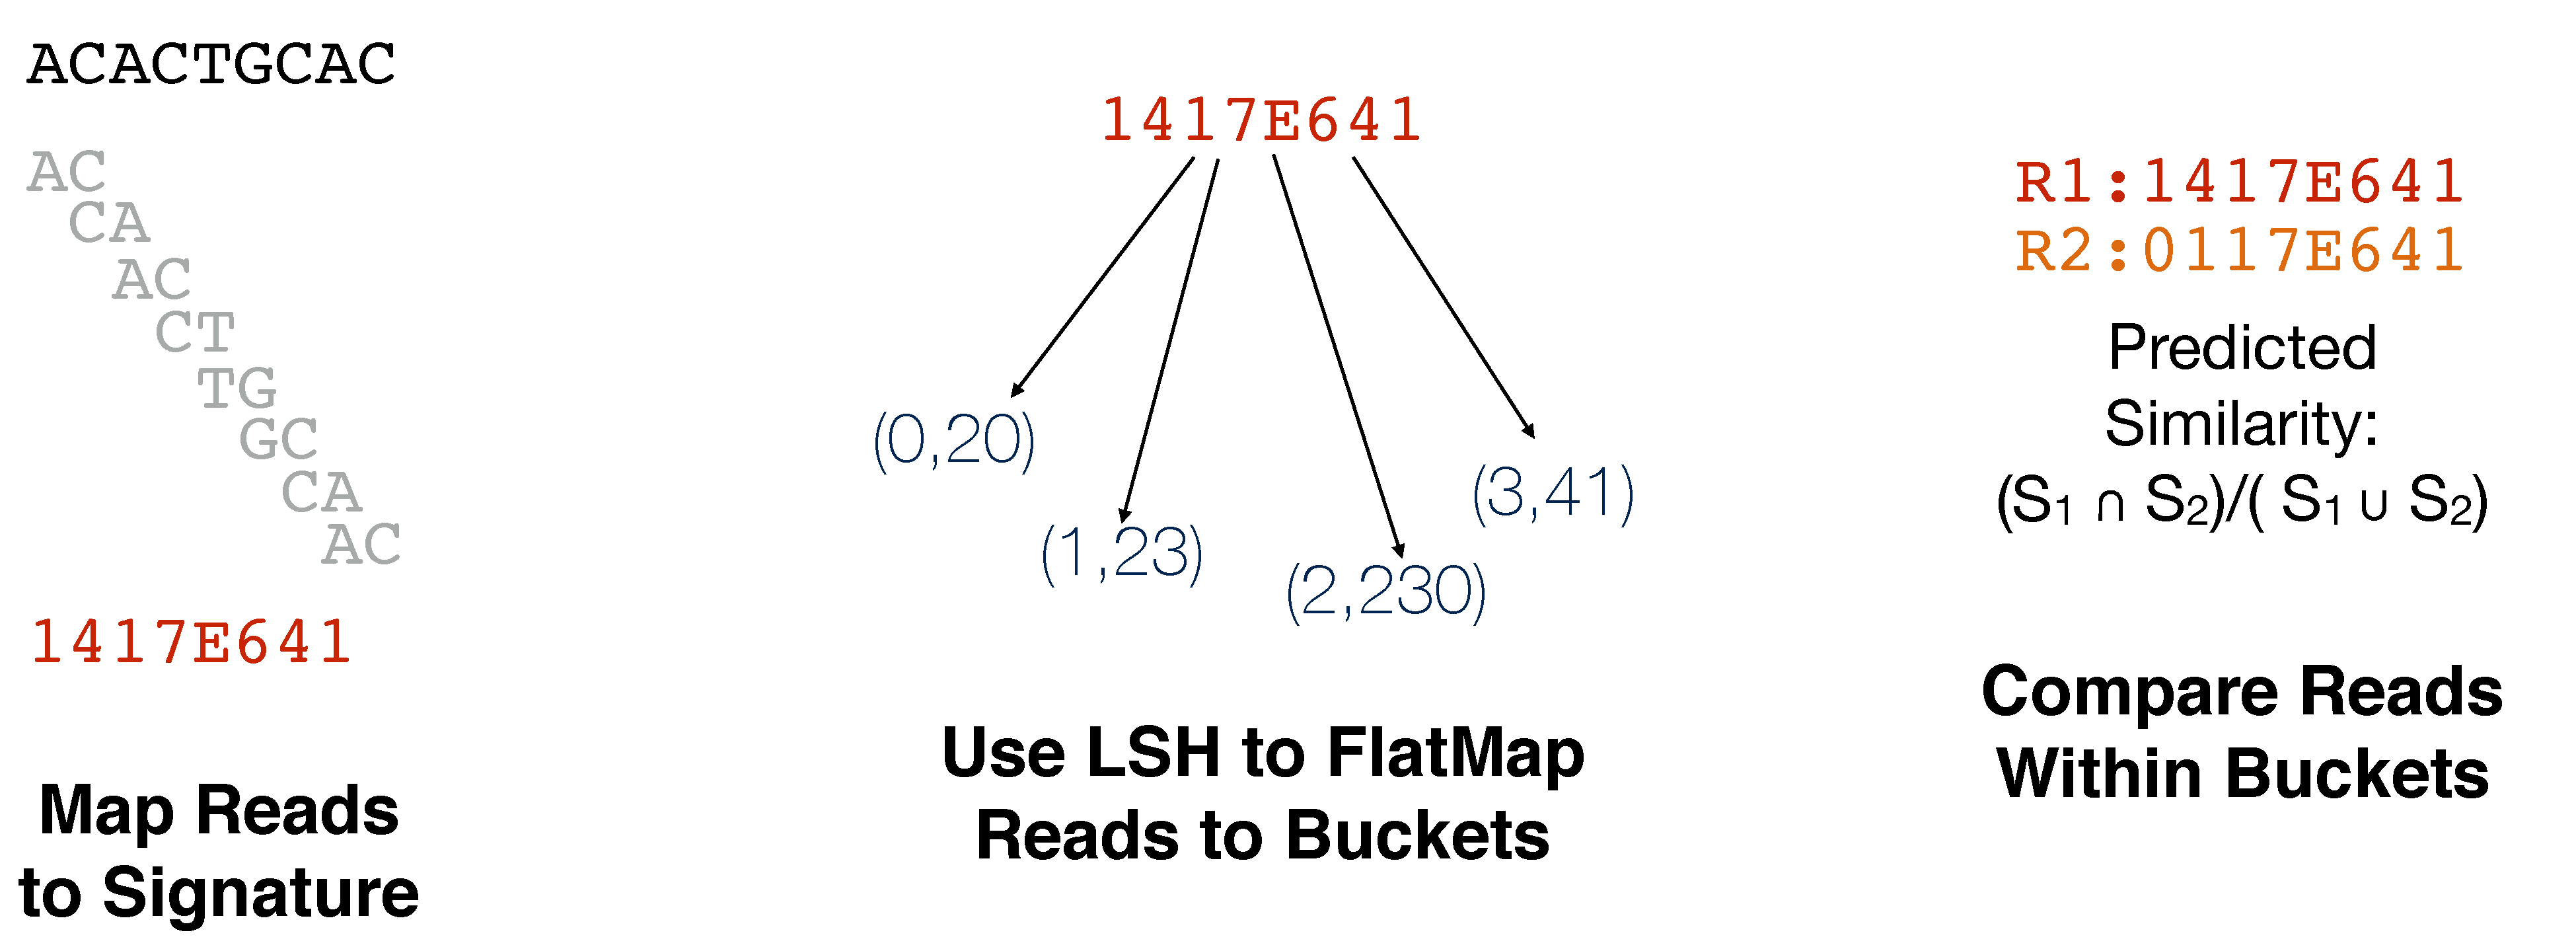
\includegraphics[width=0.95\linewidth]{minhash.pdf}
\end{center}
\end{minipage}
\pagebreak
\end{minipage}
}

\vspace{75pt}
\colorbox{Blue}{
\begin{minipage}[t]{\linewidth}
\vspace{30pt}
\begin{center}
\Huge \bf \color{White} Transitive Reduction
\end{center}
\vspace{17pt}
\end{minipage}
}
\colorbox{White}{
\begin{minipage}[t][470pt][t]{\linewidth}
\begin{minipage}{0.3\linewidth}
\LARGE
\color{Blue}
\begin{itemize}
\item Materialize all edges to vertex and use voting procedure
\item Vertices vote to keep the ``best'' edges that satisfy their reduction conditions:
\Large
\begin{itemize}
\item Final graph must keep all node-to-node \emph{paths}
\item Pick \emph{longest} edge (alignment overlap) that satisfied requirement
\end{itemize}
\end{itemize}
\end{minipage}
\begin{minipage}{0.03\linewidth}
\hfill
\pagebreak
\end{minipage}
\begin{minipage}{0.64\linewidth}
\color{Blue}
\begin{center}
\end{center}
\color{Blue}
\begin{center}
\vspace{20pt}
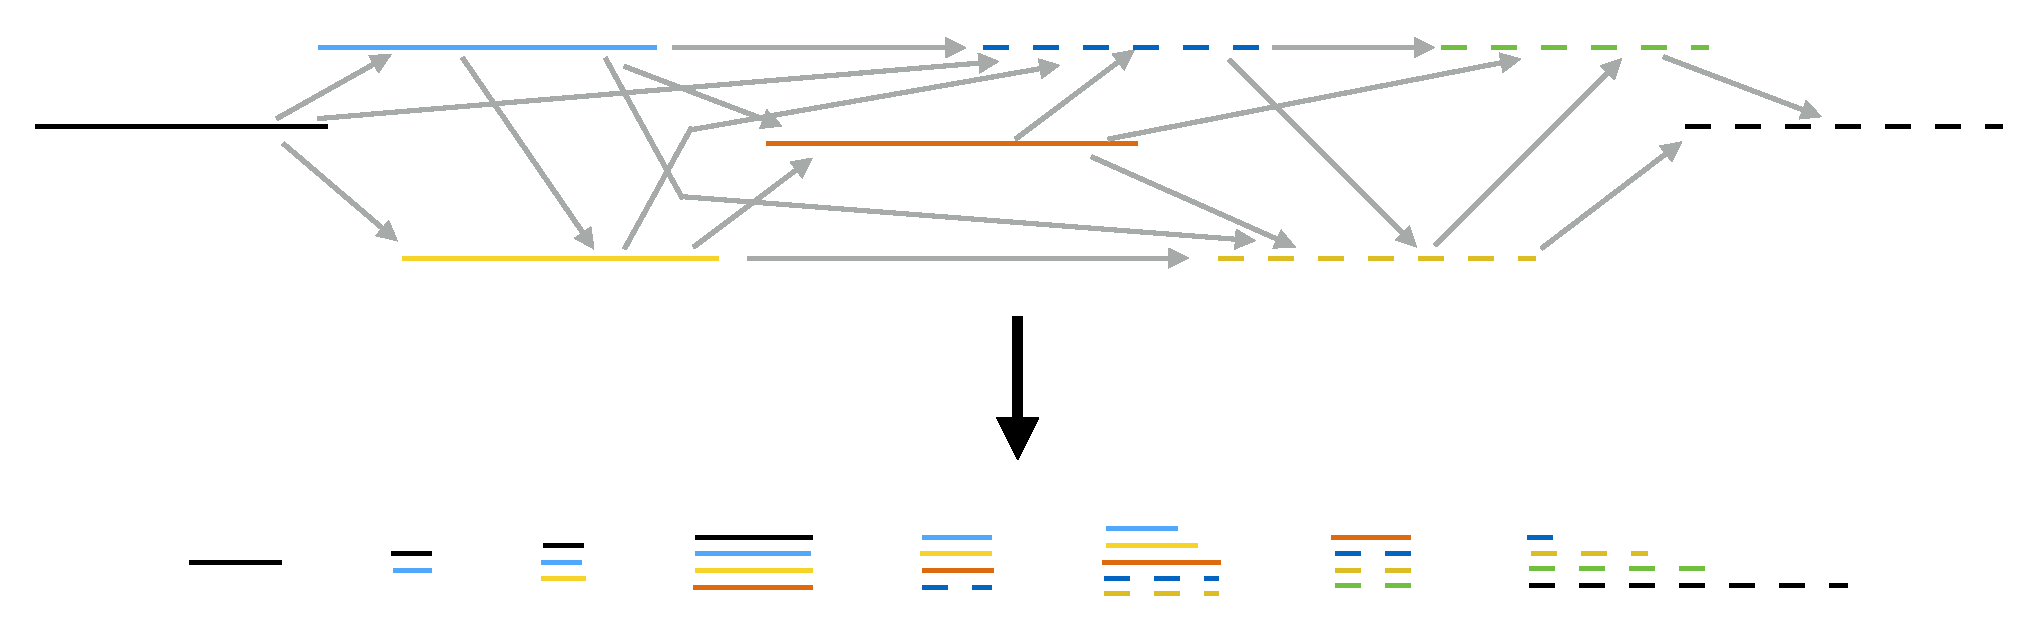
\includegraphics[width=0.9\linewidth]{transitive-reduction.pdf}
\\
Transitive Reduction Process
\end{center}
\end{minipage}
\end{minipage}
}

\vspace{75pt}
\begin{minipage}{\linewidth}
\colorbox{Blue}{
\begin{minipage}[t]{\linewidth}
\vspace{30pt}
\begin{center}
\Huge \bf \color{White} Graph Traversal
\end{center}
\vspace{17pt}
\end{minipage}
}
\colorbox{White}{
\begin{minipage}[t][480pt][t]{\linewidth}
\begin{minipage}{0.45\linewidth}
\LARGE
\color{Blue}
\begin{itemize}
\item Graph traversal is inexpensive ($\sim$5--10\% runtime)
\item Label all edges in connected component and then \texttt{groupBy} to assemble contig
\item Labeling process is complex due to bi-directed nature of edges, and uncoordinated message passing
\item Future work: add min cost flow algorithm for estimating copy number of edge/vertex
\end{itemize}
\end{minipage}
\begin{minipage}{0.03\linewidth}
\hfill
\pagebreak
\end{minipage}
\begin{minipage}{0.5\linewidth}
\color{Blue}
\begin{center}
\end{center}
\color{Blue}
\begin{center}
\vspace{20pt}
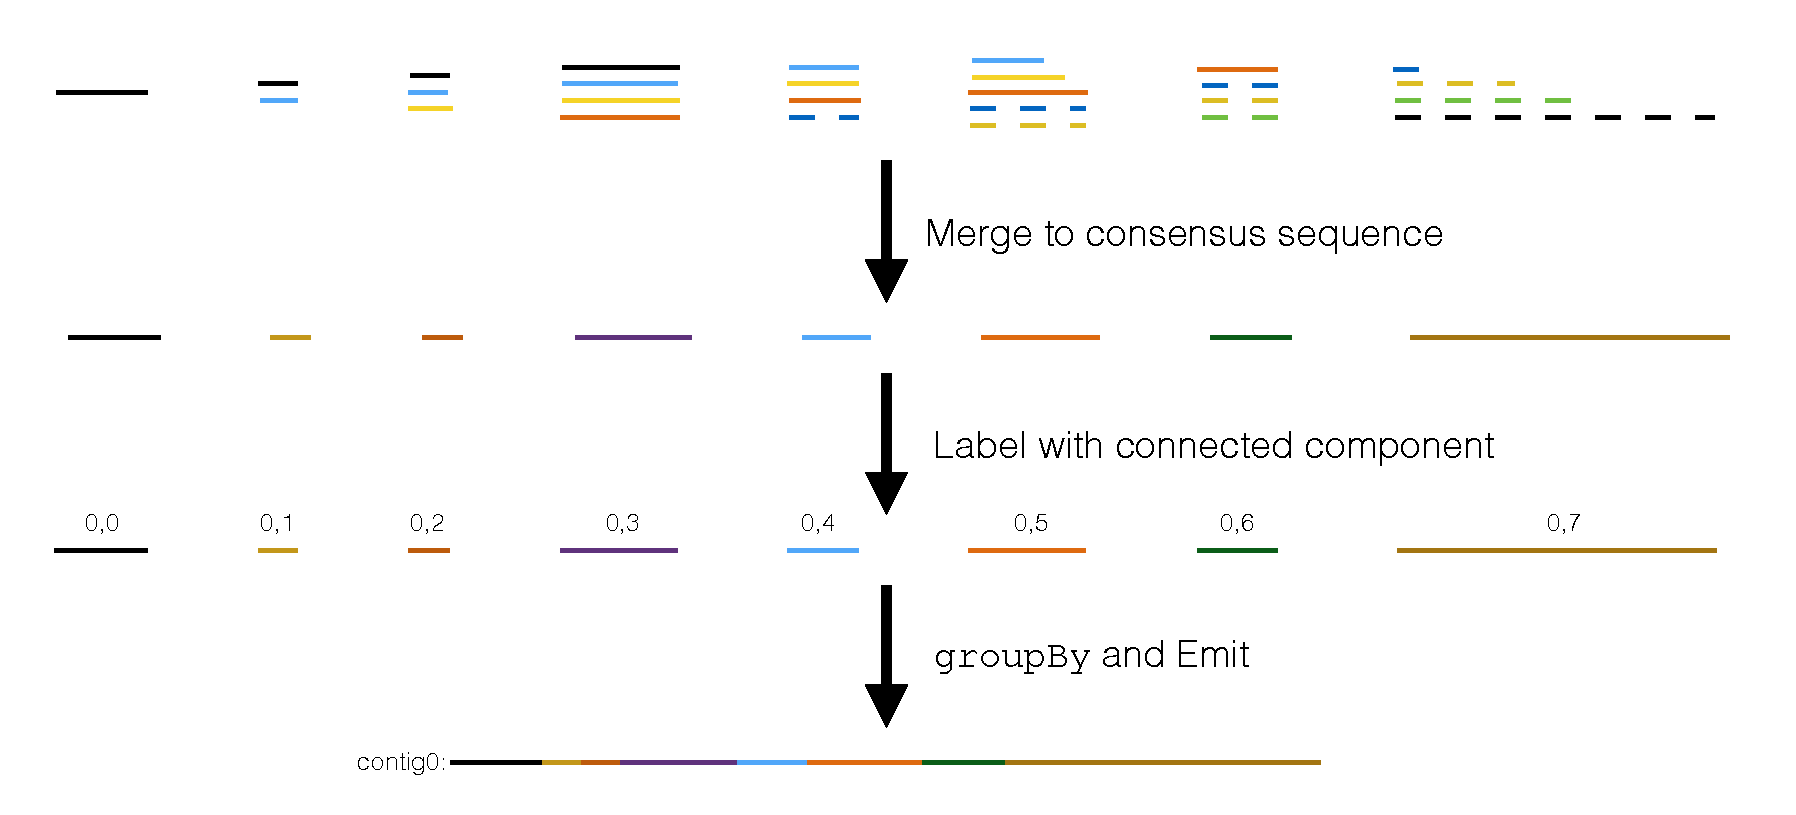
\includegraphics[width=0.9\linewidth]{walk-graph.pdf}
\end{center}
\end{minipage}
\end{minipage}
}
\end{minipage}
\end{minipage}
\end{minipage}
}

\end{document}
